% \vspace{-0.4\baselineskip}
\section{Approach}
% \vspace{-0.4\baselineskip}
\label{sec:approach}

\begin{figure*}[ht!]
\centering
% \vspace{-0.5\baselineskip}
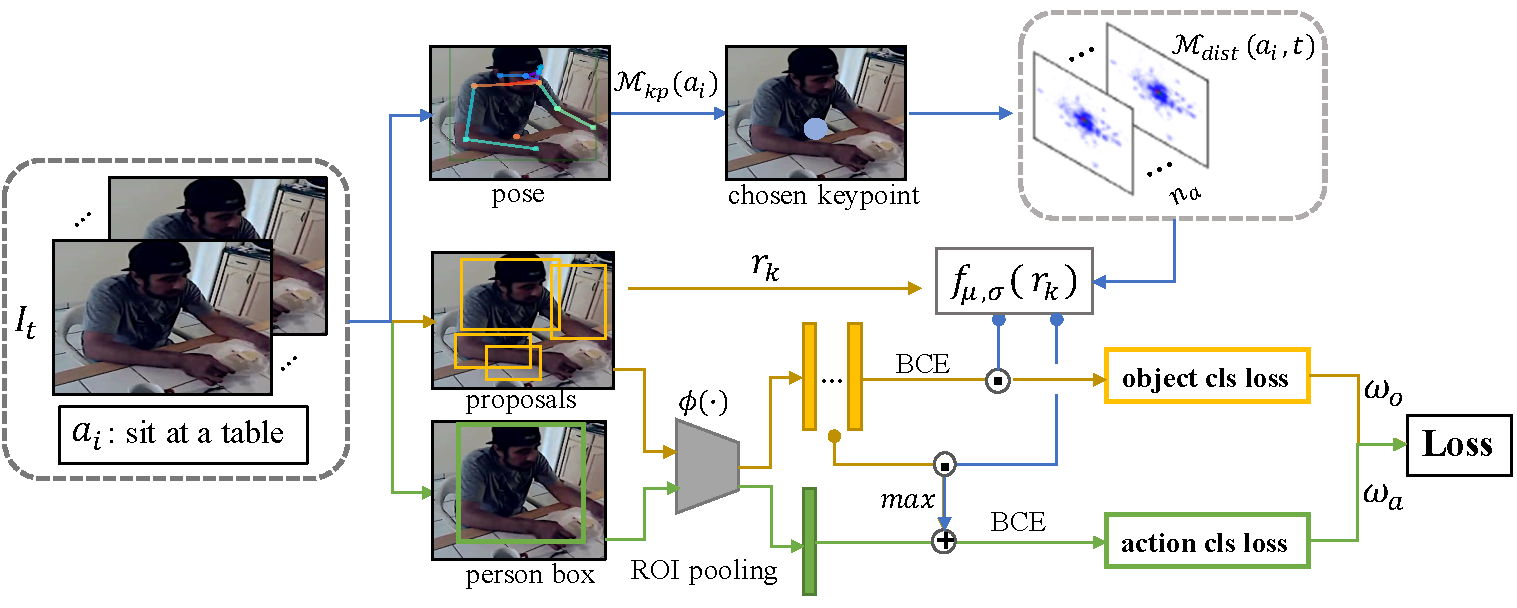
\includegraphics[width=0.8\textwidth]{figures/pipeline.pdf}
% \caption{Visual comparison of depth and normal results between \protect\cite{zhou2017unsupervised} and ours. As the original depth ground truth map comes from sparse laser measurement, the interpolated depth map is shown for better visualization. As can be seen from the depth estimation, our results preserve the small/thin structures which have similar color to other foregrounds (green circles). From the normal comparison, our results predict the road normal direction better and have no artifact. The edges in normal map are also preserved better in our results (yello circles).}
\caption{The object appearance is learned with a weakly supervised method by leveraging the three regularizations.}
% \vspace{-0.8\baselineskip}
\label{fig:pipeline}
\end{figure*}
% As discussed in \secref{sec:intro}, one major problem is that both~\cite{zhou2017unsupervised} and~\cite{yang2018aaai} have the regularization performed \wrt image gradient, which blocks nonlocal smoothness due to many false positives such as boundaries of shadows. 
In this section, we introduce the framework and different regularizations we have applied in detail.
\subsection{Overview}
% In this section, we introduce the regularizaitons we apply to learn the object representation via supervision from action labels. To better show our analysis, the information that can be leveraged are listed in different axis in \figref{fig:analysis}. Basically, we propose to explore three constraints to help learning object appearance. The first one includes the appearance consistency of objects in the same action class (blue box in \figref{fig:analysis}). The other constrain comes from the motion consistency in the same action class. The motion of ``drinking water from cup/bottle'', including both subject and object motion, is similar across videos. Last but not least, the object appears similarly in videos of different action labels but involving same object category. In the actions ``holding vacuum'' and ``fixing vacuumm'' (green box in \figref{fig:analysis}), object appearances are consistent.
As stated before, we propose to leverage appearance and motion consistency in the interaction between person and objects. The motion consistency is modeled by modeling the correlation between spatial location change with time, between person and interacted objects. Practically, such correlation is modeled between the person joint and object locations. The person joints (keypoints) are firstly estimated with off-the-shelf method and a dominant keypoint is chosen automatically by the pipeline. Attention maps around the chosen keypoint are estimated to model the probability of object locations. Class agnostic proposals are generated in a bottom-up way and weighted with the attention maps. The weighted proposals are then fed into action classification and object classification modules respectively. The action classification module takes object proposals and person detection bounding box as input and outputs action classification scores. Binary cross-entropy loss is calculated as supervision. Object classification module takes proposals as input and logistic losses are calculated for each object class as supervision. The weighted sum of the two losses is the final loss for the whole framework. 

\subsection{Framework}

Formally, for a given training video, the provided annotations include a set of action labels $\scr{L}$ = {$l_1,...,l_n$}. Each action label consists of an action class $a_i$ and corresponds to a clip in the video. The action class $a_i$ belongs to a predefined action set $a_i \in \scr{A}$, which is of size $n_{a}$: $||\scr{A}||=n_{a}$. All actions are interactive and there is one object class involved in the action $a_i\rightarrow o_{m(i)}, o_{m(i)}\in \scr{O}$. For example, object class \textit{cup} appears in the action \textit{holding a cup}. $m$ is a mapping from action class to object class. There are $n_{o}$ object classes: $||\scr{O}||=n_{o}$ in total. During training, clip-level action class $a_i$ and corresponding object class $o_j$ are used as supervision signal.

\figref{fig:pipeline} illustrates an overview of our approach. $\scr{F}$ frames are uniformly sampled from each clip and are processed with a person detector and pose estimation network to generate person bounding box $P_t$ and human key point detection results $K_t$ for each frame $f_t$. Class-agnostic proposals $R_t$ are also generated as candidate bounding boxes. To model the correlation between action and object motion, a keypoint is automatically chosen for a given action class. A spatial distribution is estimated to model the probability of object's spatial location with time. All proposals $R_t$ and person bounding box $P_t$ are processed with a convolutional network to extract appearance features. Proposal features are firstly fed into the object classification module and $n_o$-dimension classification scores are generated for each proposal region. The cross-entropy classification losses are weighted with the probability mentioned above and used as supervision from object classification. 

The action class labels are leveraged in the action classification stream. The person bounding box is processed with the same convolutional network to extract the person visual features $\phi(P_t)$. Similar to the multiple instance learning idea in \cite{gkioxari2015contextual}, the person region feaures are fused with the proposal region features $\phi(R_t)$ and then fed into the action classification module. As shown in \figref{fig:task_definition}, there may be overlap between different annotated clips, and thus it poses the action classification as a multi-label problem. The binary cross-entropy loss is used as action classification supervision. The object and action classification losses are weighted summed as the final loss term.

\subsection{Object classification}
The features are extracted for each proposal region $\phi(r_k), r_k \in R_t$ (superscript $t$ is omitted in $r_k^t$ for simpler symbol) and there are $K$ proposals on frame $f_t$: $||R_t||=K$. An $n_o$-dimensional classification score is generated by applying object classification fully connected (\textit{fc}) layer on appearance features: $S_o(r_k) = fc_o(\phi(r_k))$ for each proposal. As mentioned in the last section, there can be multiple action and object classes labels for one frame. Assume for frame $f_t$, there is a set of action labels $\scr{A}_t$ and object labels $\scr{O}_t$. Given action class $a_{i_t} \in \scr{A_t}$ and time stamp $t$, a key point is selected based on the action class $\hua{I} = \hua{M}_{kp}(a_{i_t})$ and a distribution is estimated $(\mu_{i_t}, \sigma_{i_t}) = \hua{M}_{dist}(a_{i_t}, t)$ with regard to $\scr{K}_t(\hua{I})$. $\mu_{i_t}, \sigma_{i_t} \in \scr{SE}^2$, indicating the mean and variance in 2D space respectively. Based on the estimated probability distribution $\scr{N}_{(\mu_{i_t}, \sigma_{i_t})}$ for given action class of one frame, each proposal is assigned with a probability $N_{(\mu_{i_t}, \sigma_{i_t})}(r_k), k\in [1,...,K]$. The object classification loss on frame $f_t$ is formally:
\begin{align}
\label{eqn:obj_cls_loss}
&\hua{L}_{obj} (f_t) = -\frac{1}{K\cdot |\scr{A}_t|}\sum_{a_{i_t}\in {A_t}}\sum_{k=1}^{K} N_{(\mu_{i_t}, \sigma_{i_t})}(r_k) \cdot \nonumber \\
&~~~~~~~~~~~~~~~~~~~~~~~~~~~~~~~log(P(\alpha=o_{m(i_t)}|r_k, f_t)), \nonumber\\
&P(\alpha|r_k, f_t) = \frac{exp(S_o(r_k)_{\alpha}}{\sum_{\alpha \in \scr{O}}exp(S_o(r_k)_\alpha)}, \alpha \in \scr{O}
\end{align}

\subsection{Action classification}
For the task of action recognition, especially for interactive actions as in our task, both the person and the object appearances are vital cues. As indicated in \cite{gkioxari2015contextual}, the spatial location of the most informative object, which is often the one that the person interacted with, can be mined from action recognition task. We incorporate similar idea into our pipeline by introducing a separate action classification stream to help learn the object appearance. Formally, on given frame $f_t$ in a clip, the appearance features of both person region $p$ and proposal regions $r$ are extracted and then linearly transformed into an $n_a$-dimensional score: $S_a^o(r_k) = fc_a^o(\phi(r_k))$ and $S_a^a(P_t) = fc_a^a(\phi(P_t))$. For each action class $a_{i_t} \in \scr{A}_t$, the weighted sum of proposal classification scores is added with person region classification score as a combined score. And the cross-entropy loss for each action class is averaged as the action classification loss. The formulation is shown in \equref{eqn:act_cls_loss}.

\begin{align}
\label{eqn:act_cls_loss}
&\hua{L}_{act} (f_t) = -\frac{1}{\scr{K}\cdot |\scr{A}_t|}\sum_{a_{i_t}\in {A_t}}\sum_{k=1}^{K} N_{(\mu_{i_t}, \sigma_{i_t})}(P_k) \cdot \nonumber \\
&~~~~~~~~~~~~~~~~~~~~~~~~~~~~~~~log(P(\alpha=a_{i_t}|r_k, f_t)), \nonumber\\
&P(\alpha|r_k, f_t) = \frac{exp(S_a^a(r_k)_{\alpha}+S_a^o(r_k)_{\alpha}*N_{(\mu_{i_t},\sigma_{i_t})}(r_k))}{\sum_{\alpha \in \scr{A}}exp(S_a^a(r_k)_{\alpha}+S_a^o(r_k)_{\alpha}*N_{(\mu_{i_t},\sigma_{i_t})}(r_k))}
\end{align}

\subsection{Loss terms}
The final loss is a weighted sum of the above loss terms. The hyperparameters $w_o$ and $w_a$ are weights to trade off the relative importance of object classification and action classification in the pipeline.
\begin{align}
\label{eqn:final_loss_term}
\hua{L}(\scr{F}, \scr{A}, \scr{O}) = \frac{1}{||\scr{F}||}(w_o\hua{L}_{obj}+w_a\hua{L}_{act})
\end{align}

